\documentclass{article}% For the example only, any class will do

\usepackage{tikz}
\usetikzlibrary{shapes.misc, positioning, arrows}

\usepackage{graphics}
%\pgfrealjobname{hierarchy}

\begin{document}
%\beginpgfgraphicnamed{model}
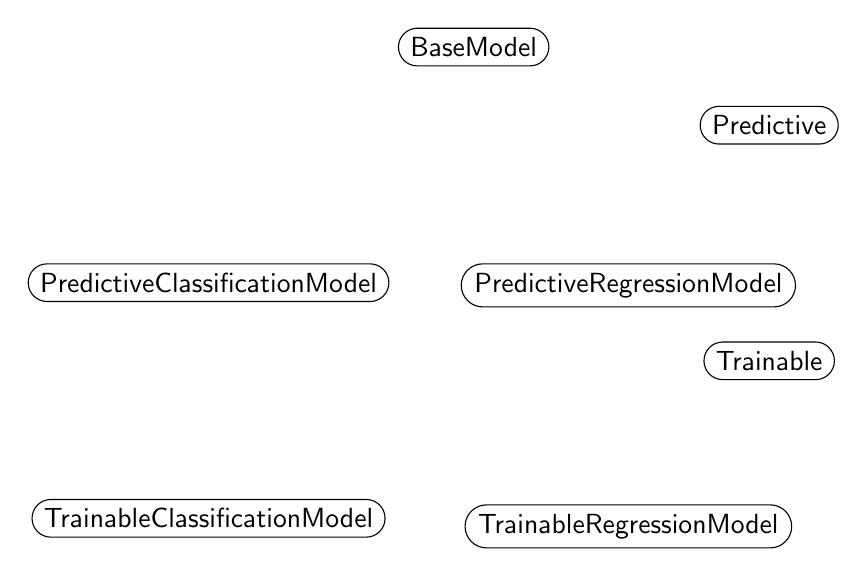
\begin{tikzpicture}[>=triangle 45,font=\sffamily]
    \node (basemodel) [draw, rounded rectangle] {BaseModel};
    \node (predictive) [below right=0.5cm and 2.4cm of basemodel, draw, rounded rectangle] {Predictive};
    \node (trainable) [below=2.5cm of predictive, draw, rounded rectangle] {Trainable};
    \node (predclassification) [below left=2.5cm and 0.6cm of basemodel, draw, rounded rectangle] {PredictiveClassificationModel};
    \node (predregression) [below right=2.5cm and -0.6cm of basemodel, draw, rounded rectangle] {PredictiveRegressionModel};
    \node (trainclassification) [below=2.5cm of predclassification, draw, rounded rectangle] {TrainableClassificationModel};
    \node (trainregression) [below=2.5cm of predregression, draw, rounded rectangle] {TrainableRegressionModel};
\end{tikzpicture}
%\endpgfgraphicnamed
\end{document}